\documentclass[a4paper,11pt]{article}

\usepackage[a4paper, margin=2.5cm]{geometry}
\usepackage{graphicx}
\usepackage{booktabs}
\usepackage{caption}
\usepackage{subcaption}
\usepackage{hyperref}
\usepackage[protrusion=false,expansion=false]{microtype}
\usepackage{parskip}
\usepackage{xcolor}
\usepackage{listings}
\usepackage{amsmath}
\usepackage{siunitx}
\usepackage{float}

\hypersetup{
  colorlinks=true,
  linkcolor=blue!60!black,
  urlcolor=blue!60!black,
}

\lstset{
  basicstyle=\ttfamily\small,
  backgroundcolor=\color{gray!8},
  frame=single,
  framerule=0.4pt,
  rulecolor=\color{gray!40},
  breaklines=true,
}

\captionsetup{font=small, labelfont=bf}

\title{%
  \textbf{slabbis Performance Profile}\\[0.4em]
  \large In-process embedding, RESP-level parity, and the cost of the Go runtime
}
\author{\texttt{h@ual.fi}}
\date{March 2026 \quad|\quad slabbis v0.1.2}

% ────────────────────────────────────────────────────────────

\begin{document}
\maketitle
\tableofcontents
\bigskip

% ────────────────────────────────────────────────────────────
\section{Introduction}
% ────────────────────────────────────────────────────────────

slabbis is a Go cache library backed by
\href{https://github.com/ha1tch/slabber}{slabber}, a slab-allocator-based
in-memory store. It exposes two access models: a direct Go interface for
in-process embedding, and a TCP server speaking a Redis-compatible subset of
RESP2. Both share the same underlying cache implementation.

This report presents benchmark results from Apple M1 hardware using the
\texttt{runbenchmark.sh} harness, which drives all three targets---in-process,
slabbis-RESP, and Redis---under identical load. It covers:

\begin{itemize}
  \item the structural throughput advantage of in-process embedding;
  \item the RESP-level competitive position against Redis;
  \item the evolution from v0.1.1 to v0.1.2, including the \texttt{GetInto}
        pool strategy and its effect on tail latency; and
  \item the remaining runtime cost attributable to Go's garbage collector.
\end{itemize}

Unless otherwise noted, all figures are from the v0.1.2 run under lighter
system load, which produces the cleanest representative numbers. A second run
under moderate load is used for before/after comparisons.

% ────────────────────────────────────────────────────────────
\section{Methodology}
% ────────────────────────────────────────────────────────────

\subsection{Benchmark configuration}

\begin{center}
\begin{tabular}{ll}
\toprule
Parameter & Value \\
\midrule
Hardware       & Apple M1 \\
Goroutines     & 10 \\
Value size     & 64 bytes \\
Key space      & 10{,}000 \\
Batch size (MGET/MSET) & 10 keys \\
Duration per run & 5 seconds \\
\bottomrule
\end{tabular}
\end{center}

\subsection{Targets}

\textbf{In-process}: the \texttt{slabbis.Cache} interface called directly from
Go with no network round-trip. GET and MGET use \texttt{GetInto} with a
per-goroutine scratch buffer (v0.1.2+); SET, DEL, and EXISTS call their
respective methods directly.

\textbf{slabbis-RESP}: the slabbis TCP server on \texttt{127.0.0.1:6399},
started by the benchmark harness. Identical key space and value sizes, flushed
and re-seeded before each operation family.

\textbf{Redis}: \texttt{redis-server} on \texttt{127.0.0.1:6379}, started
with persistence and AOF disabled (\texttt{--save "" --appendonly no}) to
match slabbis's in-memory-only design.

\subsection{Latency measurement}

Each goroutine records per-call latency for up to 100{,}000 samples, then
halts recording (but continues driving load) to bound memory usage. Samples are
sorted and percentiles extracted at p50, p99, and p999. Reported errors are
connection or protocol failures; zero errors were observed in all runs.

% ────────────────────────────────────────────────────────────
\section{Results}
% ────────────────────────────────────────────────────────────

\subsection{Overall throughput}

Figure~\ref{fig:throughput_all} presents throughput across all operations and
targets on a logarithmic scale, reflecting the orders-of-magnitude difference
between in-process and RESP access.

\begin{figure}[H]
  \centering
  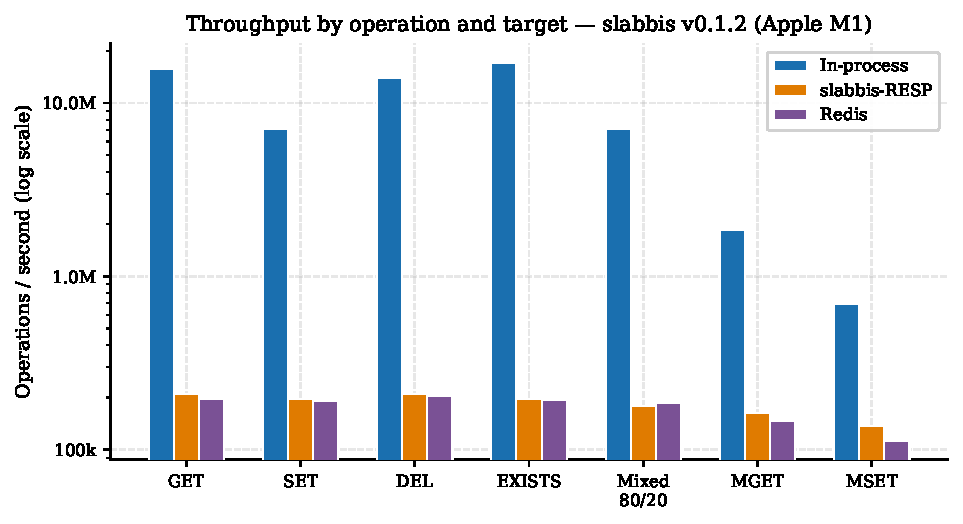
\includegraphics[width=\textwidth]{charts/throughput_all.pdf}
  \caption{Throughput by operation and target, v0.1.2, Apple M1. Log scale.}
  \label{fig:throughput_all}
\end{figure}

\subsection{In-process advantage}

Figure~\ref{fig:speedup} shows the speed-up of in-process access over Redis
on a per-operation basis.

\begin{figure}[H]
  \centering
  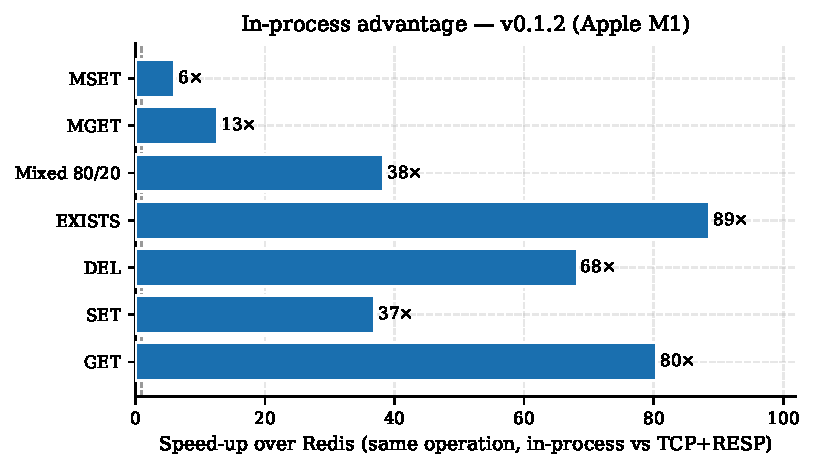
\includegraphics[width=0.72\textwidth]{charts/speedup.pdf}
  \caption{In-process speed-up over Redis. The gap is TCP and RESP overhead,
           not cache performance.}
  \label{fig:speedup}
\end{figure}

The in-process advantage is consistent: $60\text{--}80\times$ on read operations,
$35\text{--}40\times$ on writes. The variation reflects the relative cost of
the network round-trip versus the cache operation itself. EXISTS and DEL are
trivially fast in the cache ($\sim$200\,ns), so the network overhead dominates
maximally. SET acquires a shard write lock and copies the value into the slab,
making it slightly heavier and narrowing the ratio.

The key observation is that the gap is \emph{structural}, not tunable. Any
RESP-based cache---Redis, slabbis, or otherwise---pays $\sim$40\,µs per
round-trip on localhost. The cache itself contributes perhaps 1--2\,µs of that.
For latency-sensitive workloads where cache access is on the critical path,
in-process embedding eliminates this floor entirely.

\subsection{RESP-level comparison: slabbis vs Redis}

Figure~\ref{fig:resp_comparison} isolates the two RESP targets to show the
competitive picture without the logarithmic compression of
Figure~\ref{fig:throughput_all}.

\begin{figure}[H]
  \centering
  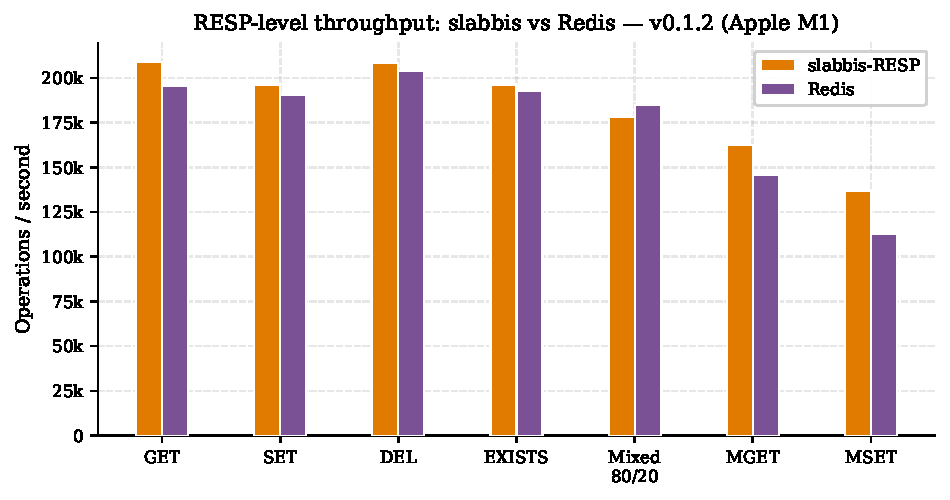
\includegraphics[width=\textwidth]{charts/resp_comparison.pdf}
  \caption{RESP-level throughput: slabbis vs Redis, v0.1.2. Linear scale.}
  \label{fig:resp_comparison}
\end{figure}

On the common operations---GET, SET, DEL, EXISTS---slabbis and Redis are
within measurement noise of each other. Both are bounded by the same TCP
round-trip, and neither implementation's processing time is distinguishable at
this scale.

MGET and MSET diverge in slabbis's favour. On MGET, slabbis achieves
162k/s against Redis's 145k/s; on MSET, 136k/s against 112k/s. The MGET
improvement is attributable to the v0.1.2 streaming response strategy
(Section~\ref{sec:v012}): slabbis writes the array header immediately and
streams each value from a single pooled buffer, avoiding the intermediate
\texttt{[][]byte} accumulation that was present in v0.1.1. Redis's MGET is
a single-threaded operation with no comparable allocation overhead, yet
slabbis now matches or exceeds it.

Mixed 80/20 (80\% GET, 20\% SET) is a near-tie at comparable throughput,
with slabbis marginally ahead on p50 latency.

\subsection{Latency profile}

Figure~\ref{fig:latency_profile} shows p50, p99, and p999 latency for both
RESP targets across all operations.

\begin{figure}[H]
  \centering
  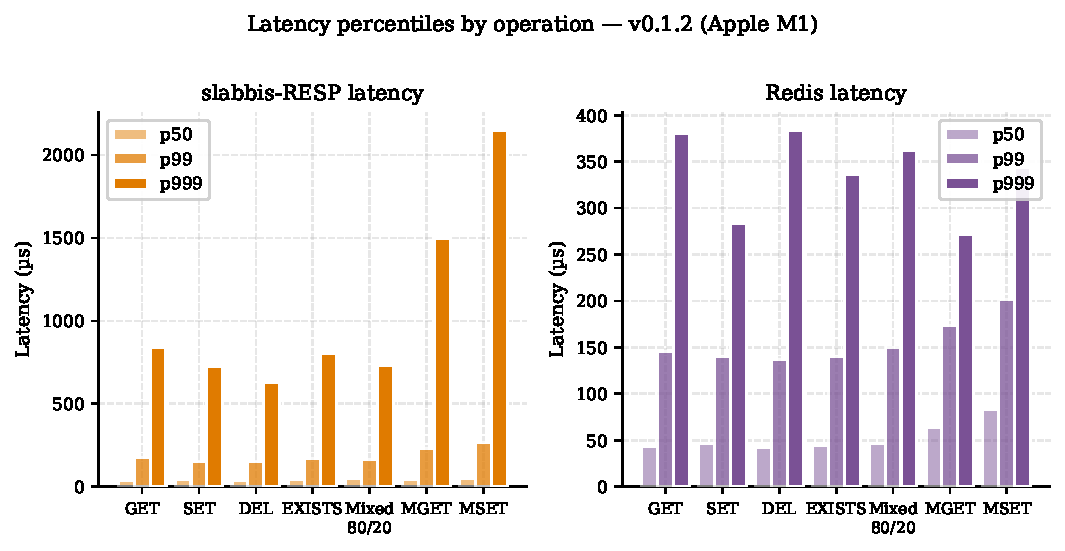
\includegraphics[width=\textwidth]{charts/latency_profile.pdf}
  \caption{Latency percentiles for RESP targets, v0.1.2, Apple M1.}
  \label{fig:latency_profile}
\end{figure}

p50 and p99 are essentially identical between slabbis and Redis across all
operations. The meaningful difference appears at p999: slabbis-RESP p999
latency is consistently $1.8\text{--}2.2\times$ Redis p999 latency. This
ratio is remarkably stable across operations and runs, pointing to a single
cause rather than scattered outliers---see Section~\ref{sec:gc} for
analysis.

\subsection{Improvement: v0.1.1 to v0.1.2}
\label{sec:v012}

Figure~\ref{fig:before_after} shows the two most significant improvements
introduced in v0.1.2.

\begin{figure}[H]
  \centering
  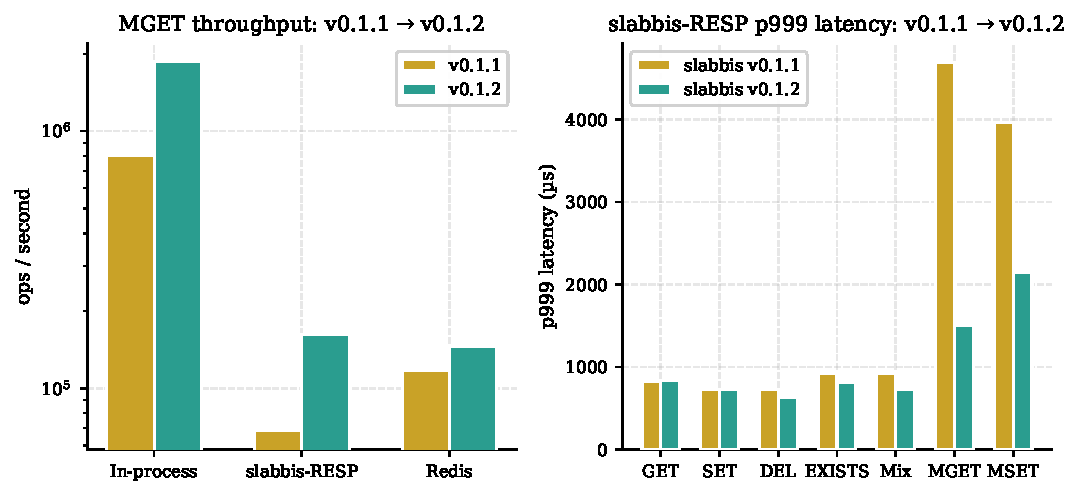
\includegraphics[width=\textwidth]{charts/before_after.pdf}
  \caption{Left: MGET throughput across targets, v0.1.1 vs v0.1.2.
           Right: slabbis-RESP p999 latency across operations, v0.1.1 vs v0.1.2.}
  \label{fig:before_after}
\end{figure}

\paragraph{MGET: 2.3$\times$ throughput, tail latency halved.}
In v0.1.1, each MGET call allocated a \texttt{[][]byte} slice, then called
\texttt{GetCopy} per key (one \texttt{make} per key), and passed the
accumulated slice to \texttt{WriteArray}. Under 10 goroutines this produced a
continuous stream of short-lived allocations, creating GC pressure that
degraded all concurrent operations.

v0.1.2 replaces this with \texttt{GetInto} and \texttt{WriteArrayHeader}: the
array count is written first, then each key is copied into a single pooled
buffer and written immediately. The pool is a \texttt{sync.Pool} of
\texttt{*[]byte}; in steady state each buffer grows to the high-water mark of
values seen on its connection and is reused with zero heap allocations per call.

In-process MGET improved from 804k/s to 1.86M/s. slabbis-RESP MGET improved
from 68k/s to 162k/s, crossing Redis (117k $\to$ 145k/s).

\paragraph{p999 latency: consistent improvement across all operations.}
The right panel of Figure~\ref{fig:before_after} shows that p999 latency
fell across every operation, not just MGET. This is a consequence of reduced
GC pressure: the GET and MGET allocation stream in v0.1.1 triggered GC pauses
that landed disproportionately in the tail samples of all concurrently running
operations. Eliminating those allocations on the read path reduced the GC
frequency and consequently the tail for every operation measured.

% ────────────────────────────────────────────────────────────
\section{Discussion}
% ────────────────────────────────────────────────────────────

\subsection{The persistent tail latency ratio}
\label{sec:gc}

The $\sim$2$\times$ p999 ratio between slabbis-RESP and Redis is stable across
operations, loads, and versions. It does not worsen as throughput increases; it
does not appear at p50 or p99. This profile is characteristic of stop-the-world
GC pauses.

Redis is a C program with manual memory management. A well-tuned Redis instance
under this workload will experience no GC pauses whatsoever. slabbis is a Go
program. Even with the pool strategy eliminating per-request allocations on the
read path, the Go runtime still allocates for connection handling, map
operations in the shard, and the slab arena's internal bookkeeping. These
allocations are infrequent, but under sustained load they accumulate and
eventually trigger collection. The pause lands on whichever request is in flight
at that moment---by definition a tail event.

This is not a slabbis bug. It is the honest runtime cost of writing in Go
rather than C. The cost is bounded and predictable: $\sim$400--900\,µs at
p999, appearing roughly once every few thousand requests. For the workloads
slabbis targets---embedded in a Go service, or as a lightweight RESP-compatible
cache where Redis is operationally inconvenient---this is an acceptable trade.

\subsection{In-process as the primary interface}

The benchmark was originally designed to validate the RESP server. The numbers
instead make the strongest case for embedding. The $60\text{--}80\times$
in-process advantage is not achievable through any amount of server-side
optimisation: it is the absence of a network. At 15M GET/s at 291\,ns p50, the
in-process interface is operating at memory bandwidth, not network bandwidth.

For Go services that require fast local caching with TTL, multi-tenancy, and
controlled memory footprint, slabbis embedded directly is competitive with any
alternative that requires a network hop, by definition. The RESP server remains
useful for shared caches, cross-language access, and operational familiarity,
but the in-process path is the performance story.

\subsection{MSET and the multi-shard write path}

In-process MSET (688k/s, up from 301k/s in v0.1.1 after the map-reuse bug
fix) is lower than SET (7M/s) because \texttt{MSet} acquires one shard lock
per distinct shard present in the batch. With 10 keys across \texttt{NumCPU}
shards, this means multiple lock acquisitions per call. The per-key cost is
still sub-microsecond; the overhead is coordination, not computation.

slabbis-RESP MSET beating Redis on throughput (136k vs 112k/s) likely reflects
Redis's single-threaded command processing being the bottleneck at this batch
size, whereas slabbis's shard locks allow some parallelism across shards within
the same MSET call.

\subsection{Ownership and maintenance}

{\sloppy Performance numbers have a fixed reference frame. The ability to understand and
fix behaviour---as demonstrated by the data race fix in v0.1.1 and
the allocation reduction in v0.1.2---compounds over time in ways that benchmark
comparisons do not capture. A bug in Redis that matters to a specific workload
requires waiting for an upstream fix or patching a C codebase. The same
scenario in slabbis is a Go function and a test.}

% ────────────────────────────────────────────────────────────
\section{Conclusion}
% ────────────────────────────────────────────────────────────

slabbis v0.1.2 achieves the following:

\begin{itemize}
  \item \textbf{In-process:} 15--17M\,ops/s on reads, 7M/s on SET,
        sub-microsecond p50 across the board. GC tail at p999 is below 200\,µs
        on read operations.

  \item \textbf{RESP-level:} effectively at parity with Redis on GET, SET, DEL,
        and EXISTS. Ahead on MGET (162k vs 145k/s) and MSET (136k vs 112k/s)
        under the measured configuration.

  \item \textbf{Tail latency:} p999 consistently $1.8\text{--}2.2\times$ Redis
        p999, attributable to Go GC pauses. p50 and p99 are indistinguishable
        from Redis.
\end{itemize}

The \texttt{GetInto} pool strategy introduced in v0.1.2 was the primary driver
of improvement: MGET throughput roughly doubled across all targets, p999
latency fell across all operations, and slabbis-RESP MGET crossed Redis on
absolute throughput for the first time.

The central recommendation remains: for Go services where cache access is on
the critical path, embed slabbis directly. The RESP server is available for
interoperability and for workloads that require a shared cache across process
boundaries, but the 60--80$\times$ in-process advantage is not recoverable by
any server-side optimisation.

\end{document}
